\chapter{UCN Production and Detection}

The first UCN at TRIUMF (Nov.~ 2017) were produced by using the
vertical UCN source described in Sec.~\ref{vertical_source}. The
spallation neutrons were converted to UCN through phonon excitation in
the isotopically pure superfluid helium.  During data taking several
measurements were performed for better understandting of the vertical
UCN source to design the next generation UCN source. In this chapter,
the experiments are described and the result are shown.

The Tungsten target is irradiated by the proton beam for a certain
amount of time. To accumulate UCN, the gate valve shown in Fig.~ (???)
must be closed during this time. A typical UCN cycle of measuremet
starts at the end of the irradiation time. After the irradiation
stops, the gate valve is opened and the UCN can reach the detector to
measure the UCN yield. When the valve is opened, the UCN rate goes up
and it eventually decays down to zero as shown in Fig.~\ref{fig:UCNRate}.

\begin{figure}[h]
  \centering
  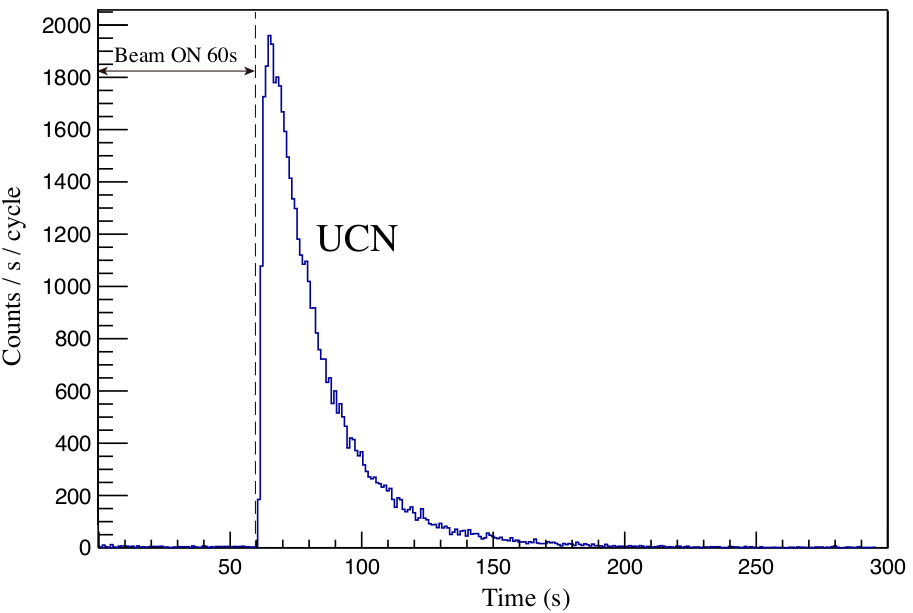
\includegraphics[width=0.7\textwidth]{UCNRate.png}
  \caption{The figure shows the UCN rate at 60~s irradiation time and
    1~$\mu$A beam current. In this case, the UCN gate valve is opened
    immediately after the end of irradiation. At this time, the UCN
    rate reaches the peak of about 2000 UCN/s. The UCN rate decays
    down to zero. The Valve is left open for 120~s. }
  \label{fig:UCNRate}
\end{figure}

The total number of produced UCN $N$ at a certain time t$_i$ can be described by
\begin{equation}
  \label{eq:totalUCN}
  N = P \tau_1\left[ 1- \exp \left(\frac{t_i }{ \tau_1}\right) \right]
\end{equation}

where $P$ is the UCN production rate and $\tau_1$ is the UCN loss rate in the source given by

\begin{equation}
  \frac{1}{\tau_1} = \frac{ f_\mathrm{He,1}}{\tau_\mathrm{He}} + \frac{1}{\tau_\mathrm{wall,1}}.
\end{equation}

Here (describe the parameters)...

First a set of UCN counts measurements is discussed. The UCN yield is
measured at different irradiation times, different beam currents and
different isotopic superfluid helium temperature. This is essential
for UCN yield optimization.  Next the UCN storage lifetime in the
source is studied at different beam currents, different irradiation
times and different temperatures of isotopically pure superfluid
helium. Over the course of the experimental run, the UCN storage
lifetime was measured on a daily basis. The idea behind this was to
look for long term changes in the source due to factors such as the
contamination in the source and to understand how long it is feasable
to run the source.






Put the rate equations here.
\section{UCN Counts Measurement}



\section{Storage Lifetime Measurements}

\section{Heater Tests of The Source}

\section{Detector Comparison}
Using the rotary valve

\section{Background Measurements}
With Ni foil

\section{UCN guide Transmission Measurements}

\section{Result And Conclusion}

%\begin{description}
%\item{I think this belongs to this chapter: UCN production by
%  multiphonon excitation in superfluid helium (I can use my candidacy
%  report for this part as a start)}
  
%\item{Some information about the detector}
  
%\item{UCN data goes here}
  
%\item{what else?}
%\end{description}
